% -*- TeX:de -*-
\NeedsTeXFormat{LaTeX2e}
\documentclass[12pt,a4paper]{article}
\usepackage[german]{babel} % german text
\usepackage[DIV12]{typearea} % size of printable area
\usepackage[T1]{fontenc} % font encoding
%\usepackage[latin1]{inputenc} % most likely on Windows
\usepackage[utf8]{inputenc} % probably on Linux
\usepackage{multicol}

% PLOTTING
\usepackage{pgfplots} 
\usepackage{pgfplotstable}
\usepackage{url}
\usepackage{graphicx} % to include images
\usepackage{tikz}
\usepackage{subfigure} % for creating subfigures
\usepackage{amsmath} % a bunch of symbols
\usepackage{amssymb} % even more symbols
\usepackage{booktabs} % pretty tables
\usepackage{makecell} % multi row table heading

% a floating environment for circuits
\usepackage{float}
\usepackage{caption}

%\newfloat{circuit}{tbph}{circuits}
%\floatname{circuit}{Schaltplan}

% a floating environment for diagrams
%\newfloat{diagram}{tbph}{diagrams}
%\floatname{diagram}{Diagramm}
\pgfplotsset{compat=1.8}
\selectlanguage{german} % use german

\begin{document}

%%%%%%% DECKBLATT %%%%%%%
\thispagestyle{empty}
			\begin{center}
			\Large{Fakultät für Physik}\\
			\end{center}
\begin{verbatim}


\end{verbatim}
							%Eintrag des Wintersemesters
			\begin{center}
			\textbf{\LARGE SS 14}
			\end{center}
\begin{verbatim}


\end{verbatim}
			\begin{center}
			\textbf{\LARGE{Physikalisches Praktikum\\ für das Bachelorstudium}}
			\end{center}
\begin{verbatim}




\end{verbatim}

			\begin{center}
			\textbf{\LARGE{PROTOKOLL}}
			\end{center}
			
\begin{verbatim}

\end{verbatim}

			\begin{flushleft}
			\textbf{\Large{Experiment (Nr., Titel): PS11 - Halleffekt in dotierten Halbleitern}}\\
							%Experiment Nr. und Titel statt den Punkten eintragen
			\LARGE{PS11 }	
			\end{flushleft}

\begin{verbatim}

\end{verbatim}	
							%Eintragen des Abgabedatums, oder des Erstelldatums des Protokolls
			\begin{flushleft}
			\textbf{\Large{Datum:}} \Large{15.05.2014}
			\end{flushleft}
			
\begin{verbatim}
\end{verbatim}
							%Namen der Protokollschreiber
		\begin{flushleft}
			\textbf{\Large{Namen:}} \Large{Patrick Braun, Johannes Kurz}
			\end{flushleft}

\begin{verbatim}


\end{verbatim}
							%Kurstag und Gruppennummer, zb. Fr/5
			\begin{flushleft}
			\textbf{\Large{Kurstag/Gruppe:}} \Large{DO/4}
			\end{flushleft}

\begin{verbatim}

\end{verbatim}
							%Name des Betreuers, das Praktikum betreute.
			\begin{flushleft}
			\LARGE{\textbf{Betreuer:}}	\Large{Wilhelm Markowitsch}	
			\end{flushleft}

%%%%%%% DECKBLATT ENDE %%%%%%%
\pagebreak
\setlength{\columnsep}{20pt}
\begin{multicols}{2}

%%%%%%%%%%%%%%%%%%%%%%%%%%%%%%%%%%%%%%%%%%%%%%%%

%\begin{figure}[H]
%	\centering
%	\includegraphics[scale=0.35]{./data/beugung.png}
%	\caption{Beugungsmuster Einzelspalt (echtes Foto; schwarz durch weiß ersetzt)}
%	\label{fig:beugungsmuster}
%\end{figure}


%\begin{figure}[H]
%	\centering
%	\pgfplotstabletypeset[
%			columns={abstand, n},
%			col sep=&,
%			columns/abstand/.style={precision=2, zerofill, column name=\makecell{$Abstand$\\$(\pm 0.05)[mm]$} }, 
%			columns/n/.style={column name=\makecell{$n$\\$(Ordnung)$}, precision=0},
%			every head row/.style={before row=\hline,after row=\hline\hline},
%			every last row/.style={after row=\hline},
%			every first column/.style={column type/.add={|}{} },
%			every last column/.style={column type/.add={}{|} }
%			]{
%			abstand & n
%			12.9 & 1
%			24.45 & 2
%			37.40 & 3
%			49.35& 4
%			62.45 & 5
%			74.45 & 6
%			87.45 & 7
%			100.25 & 8
%			
%			}
%	\caption{Messwerte Einzelspalt}
%	\label{tab:werte_einzelspalt}
%\end{figure}


%%%%%%%%%%%%%%%%%%%%%%%%%%%%%%%%%%%%%%%%%%%%%%%%
%%%%%%%%%%%%%%%%%%%%%%%%%%%%%%%%%%%%%%%%%%%%%%%%

In diesen Experimenten werden die Eigenschaften von dotierten Halbleitern in Bezug auf den Hall-Effekt untersucht. Der Hall-Effekt ist das Auftreten einer Spannung normal stehend zur Flussrichtung eines an den Halbleiter angelegten Stromes.\\


\section{Hall-Effekt in n- und p-dotiertem Germanium}
Im Halbleiter aus Germanium wird im Folgenden der lineare Zusammenhang zwischen Strom und Hallspannung überprüft.

\subsection{Grundlagen}
Grundlage der Hallspannung ist die Lorenzkraft. In ([1] p. 5 Abb. 2) ist der Aufbau der Untersuchung wie folgt zu sehen:

\begin{figure}[H]
	\centering
	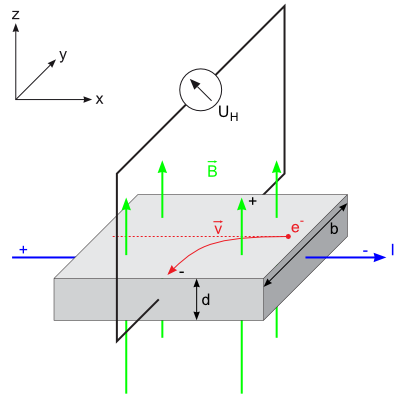
\includegraphics[scale=0.5]{./figures/hallspannung_aufbau.png}
	\caption{Entstehung der Hallspannung $U_H$ an einem stromdurchflossenen Leiter in einem Magnetfeld B.}
	\label{fig:hallspannung_aufbau}
\end{figure}

Hier ist zu sehen das normal zur Stromrichtung (in z-Richtung) das Magnetfeld angelegt wird. Normal zu Stromrichtung und normal zum Magnetfeld (Kreuzprodukt) liegt die Hallspannung an. Wie bereits erwähnt ist der Grund dafür die Lorenzkraft:

$$\vec{F_{L}} = q \cdot \vec{E} + q \cdot (\vec{v} \times \vec{B})$$



\subsection{Versuchsaufbau}





\end{multicols}
\subsection{Resultate}

%nGe UH-B
%Von x = -2,199292000000000e-01 bis x = 2,180299000000000e-01
%B (y-intercept) = 4,662737519668038e-04 +/- 1,508714424821067e-04
%A (slope) = 2,248372979857526e-01 +/- 1,124478213531423e-03
%--------------------------------------------------------------------------------------
%Chi^2/doF = 4,324795635932366e-07
%R^2 = 0,999574960134199
%Angepasstes R^2 = 0,999521830150974
%RMSE (Standardabweichung) = 0,000657631784202404
%RSS (Summe der quadrierten Restwerte) = 7,35215258108503e-06
%---------------------------------------------------------------------------------------

%nGe -I UH
%Von x = 2,000000000000000e-03 bis x = 3,000000000000000e-02
%B (y-intercept) = -1,407260213143868e-03 +/- 9,794485115681493e-04
%A (slope) = -9,434502664298404e-01 +/- 5,428232838540915e-02
%--------------------------------------------------------------------------------------
%Chi^2/doF = 1,895908081705150e-06
%R^2 = 0,983717565353814
%Angepasstes R^2 = 0,975576348030721
%RMSE (Standardabweichung) = 0,00137691978041756
%RSS (Summe der quadrierten Restwerte) = 9,47954040852575e-06
%---------------------------------------------------------------------------------------

%nGe +I UH
%
%Von x = 2,000000000000000e-03 bis x = 3,000000000000000e-02
%B (y-intercept) = -1,544205222171330e-04 +/- 2,723794209658636e-04
%A (slope) = 7,535272560696289e-01 +/- 1,505932725754159e-02
%--------------------------------------------------------------------------------------
%Chi^2/doF = 1,414480073293634e-07
%R^2 = 0,998006956474477
%Angepasstes R^2 = 0,997010434711716
%RMSE (Standardabweichung) = 0,000376095742237749
%RSS (Summe der quadrierten Restwerte) = 7,07240036646817e-07
%---------------------------------------------------------------------------------------





\begin{figure}[H]
	\centering
	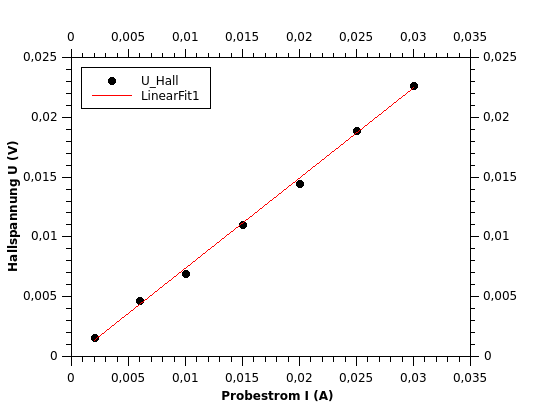
\includegraphics[scale=1.20]{./figures/Hall_nGe_+I_UH.png}
	\caption{Hallspannung mit Fit an einem n-dotierten Germaniumhalbleiter, mit positivem Strom}
	\label{fig:nGe_pI_UH}
\end{figure}
\begin{multicols}{2}



\end{multicols}
\begin{figure}[H]
	\centering
	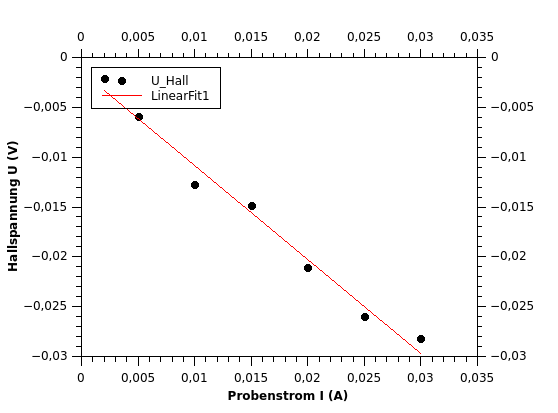
\includegraphics[scale=1.20]{./figures/Hall_nGe_-I_UH.png}
	\caption{Hallspannung mit Fit an einem n-dotierten Germaniumhalbleiter, mit negativem Strom}
	\label{fig:nGe_nI_UH}
\end{figure}
\begin{multicols}{2}



\end{multicols}
\begin{figure}[H]
	\centering
	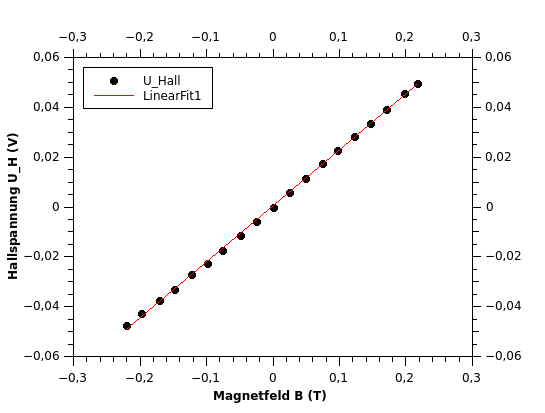
\includegraphics[scale=1.5]{./figures/Hall_nGe_UH-B.png}
	\caption{Hallspannung mit Fit bei variertem magnetischem Feld bei einem n-dotierten Germaniumhalbleiter}
	\label{fig:nGe_UH_B}
\end{figure}
\begin{figure}[H]
	\centering
	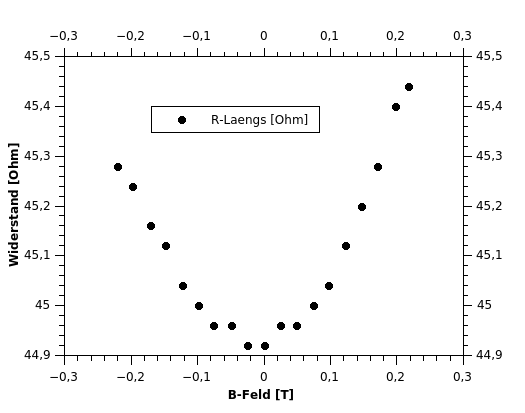
\includegraphics[scale=1.2]{./figures/Hall_nGe_magnetischer_Widerstand.png}
	\caption{Magnetowiderstand im n-Germanium}
	\label{fig:nGe_mag_wider}
\end{figure}

\begin{multicols}{2}

\noindent \textbf{Hall-Effekt im n-Ge:}\\
Probendicke $d=1mm$\\
Strom/B-Feld Proportionalität:\\
$A=(48.70 \pm 0.25)\frac{mT}{A}$\\

\noindent \emph{positive Spannungsrichtung (Abb. \ref{fig:nGe_pI_UH}):}\\

\noindent$\frac{U_H}{I_{Probe}}=(0.754\pm 0.016)V/A$\\
$I_{B-Feld}=(2.031 \pm 0.001)A$\\
$$R_H=(7620 \pm 170)\frac{cm^3}{A\cdot s}$$
$$n=(8.19\pm 0.019)\times 10^{14}cm^{-3}$$\\


\noindent \emph{negative Spannungsrichtung (Abb. \ref{fig:nGe_nI_UH}):}\\

\noindent$\frac{U_H}{I_{Probe}}=(-0.943\pm 0.016)V/A$\\
$I_{B-Feld}=(-2.059 \pm 0.001)A$\\
$$R_H=(9400 \pm 170)\frac{cm^3}{A\cdot s}$$
$$n=(6.63\pm 0.13)\times 10^{14}cm^{-3}$$\\


\noindent \emph{bei variierendem B-Feld (Abb. \ref{fig:nGe_UH_B}):}\\

\noindent$\frac{U_H}{B}=(0.2248\pm 0.0012)V/T$\\
$I_{Probe}=(25 \pm 1)mA$\\
$$R_H=(8992 \pm 370)\frac{cm^3}{A\cdot s}$$
$$n=(6.94\pm 0.29)\times 10^{14}cm^{-3}$$\\


\noindent \textbf{Magnetowiderstand (Abb. \ref{fig:nGe_mag_wider}):}\\
$\rho=(89.48\pm 0.1)\Omega \cdot cm$
$$R(B=0)=(44.92 \pm 0.05) \Omega$$
$$\mu=(0.02002 \pm 0.00084)\frac{cm^2}{Vs}$$



\pagebreak

\noindent \textbf{Hall-Effekt im p-Ge:}\\
\end{multicols}

%pGe Magnet UH
%Von x = 2,154975000000000e-01 bis x = -2,203675000000000e-01
%B (y-intercept) = -1,183992477161761e-03 +/- 3,331039840238531e-04
%A (slope) = -2,655354469324444e-01 +/- 2,493431990282161e-03
%--------------------------------------------------------------------------------------
%Chi^2/doF = 2,108132919598357e-06
%R^2 = 0,998503252811351
%Angepasstes R^2 = 0,998316159412769
%RMSE (Standardabweichung) = 0,0014519410868208
%RSS (Summe der quadrierten Restwerte) = 3,58382596331721e-05
%---------------------------------------------------------------------------------------


\begin{figure}[H]
	\centering
	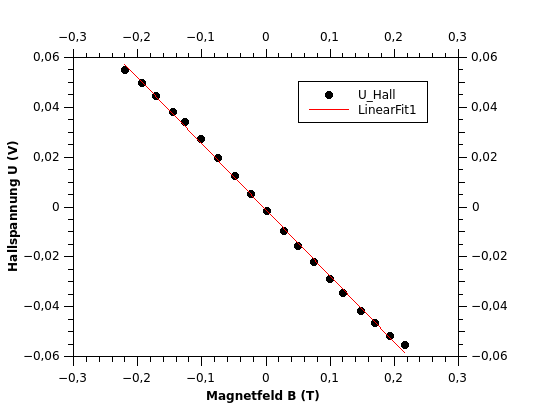
\includegraphics[scale=1.3]{./figures/Hall_pGe_UH-B.png}
	\caption{Hallspannung mit Fit bei variertem magnetischem Feld bei einem p-dotierten Germaniumhalbleiter}
	\label{fig:pGe_UH_B}
\end{figure}

\begin{figure}[H]
	\centering
	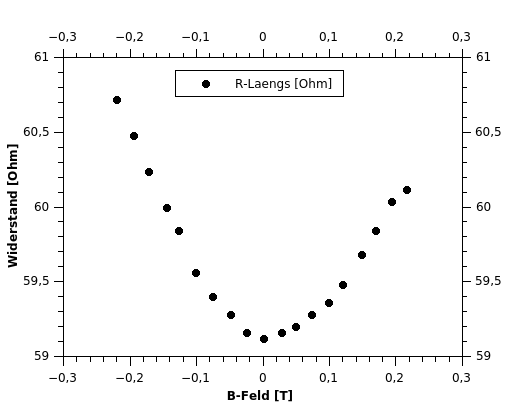
\includegraphics[scale=1.3]{./figures/Hall_pGe_magnetischer_Widerstand.png}
	\caption{Magnetowiderstand im p-Germanium}
	\label{fig:pGe_mag_wider}
\end{figure}
\begin{multicols}{2}


\noindent \emph{bei variierendem B-Feld (Abb. \ref{fig:nGe_UH_B}):}\\

\noindent$\frac{U_H}{B}=(-0.2655 \pm 0.0025)V/T$\\
$I_{Probe}=(25 \pm 1)mA$\\
$$R_H=(-10620 \pm 440)\frac{cm^3}{A\cdot s}$$
$$p=(5.88\pm 0.25)\times 10^{14}cm^{-3}$$\\

\noindent \textbf{Magnetowiderstand (Abb. \ref{fig:pGe_mag_wider}):}\\
$\rho=(118.24 \pm 0.1)\Omega \cdot cm$
$$R(B=0) = (59.12 \pm 0.05)\Omega$$
$$\mu=(0.01795 \pm 0.00077)\frac{cm^2}{Vs}$$



Rohdaten sind zu finden unter [2].

\subsection{Diskussion}

Sowohl in den Messungen des Hall-Effekts im n-Germanium (Abb. \ref{fig:nGe_pI_UH}, Abb. \ref{fig:nGe_nI_UH} und Abb. \ref{fig:nGe_UH_B}) als auch im p-Germanium (Abb.\ref{fig:pGe_UH_B}) ist die lineare Abhängigkeit des Effekts vom Strom durch die Probe sowie dem angelegten Magnetfeld, gut zu sehen.\\
Auch zu sehen ist, dass positive und negative Ladungsträger (n-Ge, p-Ge) in die gleiche Richtung abgelenkt werden, bei gleichbleibender Orientierung des B-Feldes bzw. des Stromes. (Der Vorzeichenwechsel der Ladung wird kompensiert durch den Vorzeichenwechsel der Ladungsflussrichtung).\\
Auch die Abhängigkeit des Widerstandes der Probe vom angelegten Magnetfeld konnte gezeigt werden (Abb.\ref{fig:nGe_mag_wider} und Abb. \ref{fig:pGe_mag_wider}).\\
Qualitativ stimmen beide Kurven auch mit dem Modell überein (quadratische Abhängigkeit des Widerstandes vom B-Feld)

Noch genauer zu betrachten ist, dass die Ladungsträgerdichten p und n (die sich direkt aus der Hallkonstante $R_H$ errechnen) zwar für alle Aufbauten in der gleichen Größenordnung liegen, jedoch deutlich unterschiedlich sind (außerhalb ihrer Unsicherheiten).\\
Da die genaue Beschaffenheit der Proben nicht bekannt ist, ist das für dir p-Germanium-Probe durchaus plausibel (da hier ja nur die magnetfeldabhängige Messung durchgeführt wurde, also kein direkter Vergleichswert besteht).\\
Der fest verlötete Messaufbau mit den Abstandhaltern für die Magneten scheint wenig Spielraum für systematische Fehler/ Verbesserungen zu bieten. Auch die verwendeten Messgeräte sind, nach Herstellerangabe und bisherigen Erfahrungen (Fluke) hinreichend genau.\\
Eine mögliche Ursache sind Temperaturschwankungen im Halbleiter, je nach Strom und Widerstand. Dieser ist schließlich auch vom B-Feld abhängig. Da doch ein großer Bereich an verschiedenen Strömen durch die Proben fließt, dürfte das eine plausible Ursache für die größere Unsicherheit sein.\\
Eine einfache Temperaturmessung (während der Aufgaben, die noch nicht die Temperaturabhängigkeit darstellen sollen) könnte hier Aufschluss geben. Möglicherweise führt eine andere Gruppe diese durch.\\
Andere Möglichkeiten bleiben, dass die Abmessungen der Probe als fehlerfrei angenommen wurden, sowie der Magnetowiderstand, obgleich er bestimmt wurde, noch nicht bei der Betrachtung der Hall-Konstanten berücksichtigt wurde.



\section{Temperaturabhängigkeit des Hall-Effekts}

\subsection{Grundlagen und Versuchsaufbau}
In diesem Versuch soll die Temperaturabhängigkeit des Hall-Effekts gezeigt werden.\\
Dazu ist in der verwendeten Schaltung der beiden Germanium-Proben jeweils zusätzlich ein Heizelement und ein Anschluss zur Temperaturmessung angebracht. Die Messung selbst wird computergestützt durchgeführt und lässt sofort die Abhängigkeit von Längsspannung und Hallspannung von der Temperatur erkennen.\\

Es wird erwartet, dass die Spannung (proportional zum Widerstand bei konstantem Strom) im unteren Temperaturbereich bis zu einer gewissen Temperatur linear steigt, bis zu einem Wendepunkt, an dem sie exponentiell abfällt.\\
Nahe der Raumtemperatur überwiegt nämlich ein metallischer Charakter des Halbleiters:\\
Es ist eine gewisse Anzahl Elektronen im  Leitungsband und damit frei bewegliche Ladungsträger im Material. Wird dieses nun wärmer, behindert die höhere Energie der Atomrümpfe deren Bewegung, damit steigt der Widerstand (linear wie eben in Metallen).\\
Gleichzeitig übernimmt aber, mit steigender Temperatur, die Halbleitercharakteristik: Eine zunehmende Menge Ladungsträger (abhängig von der Dotierung) gelangen in das Leitungsband. Die Leitfähigkeit nimmt also zu (und damit die Spannung und der Widerstand ab).\\
Dieser Prozess sollte, wie eben in der Temperaturabhängigkeit von Halbleitern (PW10) gezeigt, exponentiell verlaufen und damit schnell zum bestimmenden Faktor der Leitfähigkeit werden.





\subsection{Resultate}


 




\noindent Die Rohdaten sind zu finden unter [2].

\subsection{Diskussion}


\section{Quellen}
$[1]$ Anleitung, \url{http://www.univie.ac.at/anfpra/neu1/ps/ps11/PS11.pdf}\\
$[2]$ Rohdaten, \url{htts://github.com/blackandcold/Protocols-SS2014-P2/tree/master/PS_11/daten}\\

\end{multicols}
\end{document}